\documentclass[12pt]{article}
\setlength{\oddsidemargin}{0in}
\setlength{\evensidemargin}{0in}
\setlength{\textwidth}{6.5in}
\setlength{\parindent}{0in}
\setlength{\parskip}{\baselineskip}

\usepackage{amsmath,amsfonts,amssymb,bm,graphics,pgfplots,framed,dsfont}
\usepackage[scale=0.75,top=1cm,bottom=3cm]{geometry}

\begin{document}

\textbf{Minh Anh Nguyen }\\
\textbf{Discrete Math\hfill Test Sample}

\hrulefill

\begin{enumerate}
  %--%
  \item Write a proof sequence for the following assertion. Justify each step.
        \begin{center}
            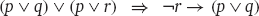
\includegraphics[scale=2.5]{img/img-0.png}
        \end{center}
  \item Let the following predicates be given. The domain is all cars.
  \[\text{F(x) = x is fast}\]
  \[\text{S(x) = x is a sports car}\]
  \[\text{E(x) = x is expensive}\]
  \[\text{A(x,y) = x is safer than y}\]
        \begin{enumerate}
            \item Write the following statements in predicate logic.
            \begin{enumerate}
                \item All sports cars are fast.
                \item There are fast cars that aren’t sports cars.
                \item Every fast sports car is expensive.
            \end{enumerate}
            \item Write the following predicate logic statement in everyday English. Don’t just give a word-for-word translation; your sentence should make sense.
            \begin{center}
                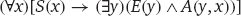
\includegraphics[scale=2.5]{img/img-1.png}
            \end{center}
            \item Formally negate the statement from part (b). Simplify your negation so that no quantifier or connective lies within the scope of a negation. State which derivation rules you are using.
        \end{enumerate}
    \item Recall Example 2.1. The diagram below shows modern-day Kaliningrad, in which two of the bridges from Euler’s day no longer exist. Represent these five bridges and four land masses as an undirected graph. Is it possible to travel an Euler path on this graph? Why or why not?
    \begin{center}
        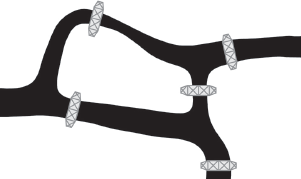
\includegraphics[scale=2.5]{img/img-3.png}
    \end{center}

    \newpage    

    \item Let A, B, and C be sets, and let $X = A \cup B$.
    \begin{enumerate}
        \item Write $|X \cap C|$ in terms of $|A \cap C|$, $|B \cap C|$, and $|A \cap B \cap C|$. Hint: In the following Venn diagram, $X \cap C$ is the shaded area.
        \begin{center}
            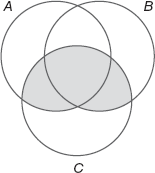
\includegraphics[scale=0.7]{img/img-4.png}
        \end{center}
        \item Write $|A \cup B \cup C|$ in terms of $|A|$, $|B|$, $|C|$, $|A \cap B|$, $|A \cap C|$, $|B \cap C|$, and $|A \cap B \cap C|$. (The result is the inclusion–exclusion principle for three sets.)
    \end{enumerate}

    \item List all the elements of P(P({1})).
    \item The following set R defines an equivalence relation on the set \{1, 2, 3\}, where a R b means that $(a, b) \in R$.
        \begin{center}
            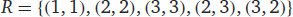
\includegraphics[scale=3]{img/img-5.png}
        \end{center}
        What are the equivalence classes?

    \item Give a specific reason why the following set R does not define an equivalence relation on the set \{1, 2, 3, 4\}.
    \begin{center}
        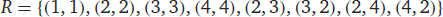
\includegraphics[scale=3]{img/img-6.png}
    \end{center}

    \item Let S = \{1, 2, 3, 5, 10, 15, 20\}. It is a fact that (S, |) is a poset. Draw its Hasse diagram.
    \item The following graph has 45 vertices.
    \begin{center}
        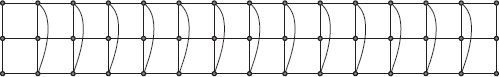
\includegraphics[scale=2]{img/img-7.png}
    \end{center}
    \begin{enumerate}
        \item Does this graph have an Euler circuit? Why or why not?
        \item Does this graph have an Euler path? Why or why not?
        \item The graph below is a copy of the above graph, but with some additional edges added so that all of the vertices in the resulting graph have degree four.
        \begin{center}
            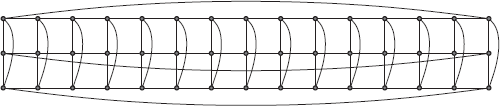
\includegraphics[scale=2]{img/img-8.png}
        \end{center}
        How many edges does this new graph have? Explain how you can use a theorem from this section to make counting the edges easier.
    \end{enumerate}

    \item Is $1 + \frac{17}{6}n - 2n^2 + \frac{7}{6}n^3$ a closed-form solution for the following recurrence relation? Prove or disprove.
    \begin{center}
        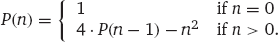
\includegraphics[scale=3]{img/img-9.png}
    \end{center}

    \item How many solutions (using only nonnegative integers) are there to the following equation?
    \[x_1 + x_2 + x_3 + x_4 + x_5 + x_6 + x_7 = 20  \]

\end{enumerate}
\end{document}